\documentclass[8pt]{beamer}
\usepackage[utf8]{inputenc}
\usepackage{xeCJK}
\usepackage{graphicx}
\usepackage {mathtools}
\usepackage{utopia} %font utopia imported
\usetheme{CambridgeUS}
\usecolortheme{dolphin}

% set colors
\definecolor{myNewColorA}{RGB}{255,102,0}
\definecolor{myNewColorB}{RGB}{255,163,102}
\definecolor{myNewColorC}{RGB}{255,224,204}
\setbeamercolor*{palette primary}{bg=myNewColorC}
\setbeamercolor*{palette secondary}{bg=myNewColorB, fg = white}
\setbeamercolor*{palette tertiary}{bg=myNewColorA, fg = white}
\setbeamercolor*{titlelike}{fg=myNewColorA}
\setbeamercolor*{title}{bg=myNewColorA, fg = white}
\setbeamercolor*{item}{fg=myNewColorA}
\setbeamercolor*{caption name}{fg=myNewColorA}
\usefonttheme{professionalfonts}
\usepackage{natbib}
\usepackage{hyperref}
%------------------------------------------------------------
\titlegraphic{
\includegraphics[height=2cm]{figures/nus_logo_full-horizontal.jpg}}

\setbeamerfont{title}{size=\LARGE}
\setbeamerfont{subtitle}{size=\normalsize}
\setbeamerfont{author}{size=\normalsize}
\setbeamerfont{date}{size=\normalsize}
\setbeamerfont{institute}{size=\normalsize}
\title[National University of Singapore]{\textbf{Certifiably Optimal Rotation And Pose Estimation Based On The Caylay Map}}
% \subtitle{Some Subtitle}
\author[cchenyu]{Cao Chenyu}
\institute[c.chenyu@u.nus.edu]{National University of Singapore}
\date[ME5419 Presentation]{\today}

%------------------------------------------------------------
\usepackage{tikz}
\usepackage{wrapfig}
\setbeamertemplate{caption}[numbered]
% \usepackage{times}
\setlength{\abovedisplayskip}{5pt}
\setlength{\belowdisplayskip}{5pt}
\setlength{\abovedisplayshortskip}{2pt}
\setlength{\belowdisplayshortskip}{2pt}
%------------------------------------------------------------

\begin{document}

%The next statement creates the title page.
\frame{\titlepage}
% \begin{frame}
% \frametitle{Contents}
% \tableofcontents
% \end{frame}
%------------------------------------------------------------
\section{Introduction}
\begin{frame}{Introduction}

State estimation is concerned with fusing several noisy measurements into a less noisy estimate, while the vector itself may \textbf{not in a vector space} (e.g. rotation matrix), which means that it is a \textbf{non-convex problem}.\\
\vspace{1em}
As shown in Fig. \ref{fig:non-convex}, non-convex problems are difficult to solve (than convex ones) because they have \textbf{local minima} and common gradient-based opimizers can easily become trapped, which means that we usually need a good \textbf{initial guess} for \texttt{x} to arrive at the global minimum. What if such an intial guess is not available?
\begin{figure}
    \centering
    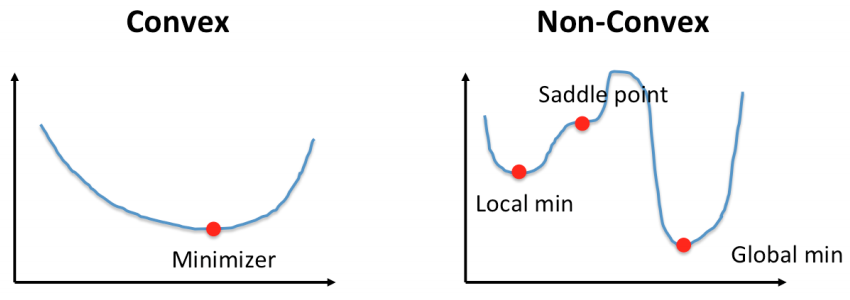
\includegraphics[width=0.7\textwidth]{figures/nonvex.jpg}
    \caption{convex vs. non-convex}
    \label{fig:non-convex}
\end{figure}


\end{frame}

\section{Mathematical Background}
\begin{frame}{Lie Groups for Rotations and Poses}
The \textit{special orthogonal group}, representing rotations, is the set of valid rotation matrices:
\begin{equation}
SO(3) = \{ C \in \mathbb{R}^{3 \times 3} | CC^T = I, \det(C) = 1 \}
\end{equation}
where \( I \) is the identity matrix. It is common to map a vector, \( \boldsymbol{\phi} \in \mathbb{R}^3 \), to a rotation matrix, \( C \), through the matrix exponential.
\begin{equation}
    C(\boldsymbol{\phi}) = \exp (\boldsymbol{\phi}^\wedge),
    \boldsymbol{\phi}^\wedge = 
\begin{bmatrix}
\phi_1 \\
\phi_2 \\
\phi_3 
\end{bmatrix}
^\wedge = 
\begin{bmatrix}
0 & -\phi_3 & \phi_2 \\
\phi_3 & 0 & -\phi_1 \\
-\phi_2 & \phi_1 & 0 
\end{bmatrix}
\end{equation}
The \textit{special Euclidean group}, representing poses (i.e., translation and rotation), is the set of valid transformation matrices:
\begin{equation}
SE(3) = \left\{ T = \begin{bmatrix} C & r \\ \mathbf{0}^T & 1 \end{bmatrix} \in \mathbb{R}^{4 \times 4} \mid C \in SO(3), r \in \mathbb{R}^3 \right\}    
\end{equation}
It is again common to map a vector, \( \boldsymbol{\xi} \in \mathbb{R}^6 \), to a transformation matrix, T \( \in SE(3) \), through the matrix exponential.

\begin{equation}
T(\xi) = \exp(\xi^{\wedge}),
\xi^{\wedge} = \begin{bmatrix} \mathbf{p} \\ \boldsymbol{\phi} \end{bmatrix}^{\wedge} = \begin{bmatrix} \boldsymbol{\phi}^{\wedge} & \mathbf{p} \\ \mathbf{0}^T & 0 \end{bmatrix}.
\end{equation}

\end{frame}

\section{Mathematical Background}
\begin{frame}{Cayley Map}
Cayley map is another way to map from a Lie algebra (vector space) to a Lie group. We can write the rotation matrix in terms of the Cayley map (Cayley map can also be used to map pose vectors to \textit{SE(3)}):
\begin{equation}
C(\phi) = \text{cay}(\phi^\wedge) = \left( I - \frac{1}{2} \phi^\wedge \right)^{-1} \left( I + \frac{1}{2} \phi^\wedge \right),
\end{equation}
\begin{equation}
\phi = \text{cay}^{-1}(C)^\vee = (2(C - I)(C + I)^{-1})^\vee
\end{equation}

\begin{figure}
    \centering
    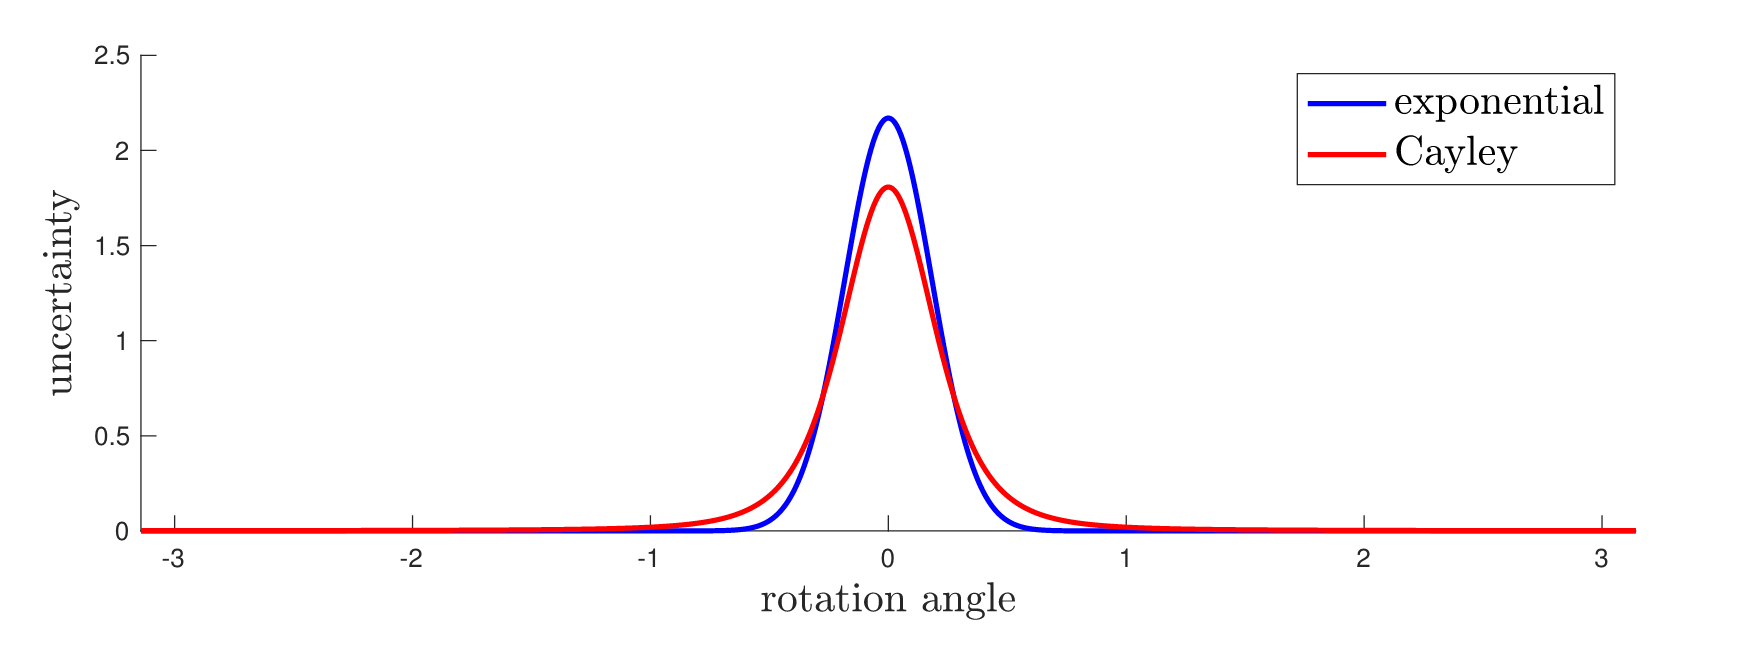
\includegraphics[width=0.6\textwidth]{figures/cayley_vs_exp.png}
    \caption{Comparison of uncertainty on rotation angle for the exponential and Cayley maps}
    \label{fig:caylet_vs_exp}
\end{figure}

As shown in Fig. \ref{fig:caylet_vs_exp}, the two distributions are nearly identical for small uncertainty. In this paper the Cayley map is used to achieve global optimality through the use of convex relaxations.

\end{frame}

\section{Convex Relaxation}
\begin{frame}{Convex Relaxation}
\begin{columns}[T]
\begin{column}{0.48\textwidth}
Suppose a non-convex optimization problem of the form:
\begin{equation}
\begin{aligned}
\min \quad & f(z) \\
\text{w.r.t.} \quad & Z \\
\text{s.t.} \quad & g_i(Z) = 0 \quad \forall i
\end{aligned}
\end{equation}
Quadratically Constrained Quadratic Program (QCQP) (still nonconvex).
\begin{equation}
\begin{aligned}
\text{min} \quad & \text{tr}(QX) \\
\text{w.r.t.} \quad & X \\
\text{s.t.} \quad & X \succeq 0 \\
& \text{rank}(X) = 1 \\
& \text{tr}(A_0 X) = 1 \\
& \text{tr}(A_i X) = 0 \quad (\forall i \neq 0)
\end{aligned}
\end{equation}
\end{column}

% \begin{tikzpicture}[overlay, remember picture]
%   \draw[dashed, red] ([yshift=-1.5cm]current page.north) -- ([yshift=0.7cm]current page.south);
% \end{tikzpicture}

\begin{column}{0.48\textwidth}
Drop rank(X) = 1 constraint, we have a convex relaxation of the problem in the form of of a Semidefinite Program (SDP):
\begin{equation}
\begin{aligned}
\text{min} \quad & \text{tr}(QX) \\
\text{w.r.t.} \quad & X \\
\text{s.t.} \quad & X \succeq 0 \\
& \text{tr}(A_0 X) = 1 \\
& \text{tr}(A_i X) = 0 \quad (\forall i \neq 0)
\end{aligned}
\end{equation}
Unfortunately, this relaxation is still not tight for most problems in this paper, then \textbf{redundant constraints} are introduced in order to tighten it. (In the concurrency work they have been developing the tools to find such constraints.)
\begin{equation}
\text{(redundant)} \quad \text{tr}(B_j X) = 0 \quad (\forall j \neq 0)
\end{equation}
\end{column}
\end{columns}
\end{frame}

\section{Averaging}
\begin{frame}{Rotation Averaging}

The trouble of the matrix exponential and logarithm is that they are difficult expressions to manipulate into QCQP. Thus, we can use the Caylay map to simply 'average' several noisy estimates of rotation or pose:

\begin{equation}
\begin{aligned}
& \text{min} \quad \sum_{m=1}^{M} \text{cay}^{-1} \left( C \tilde{C}^T_m \right)^{\vee^T} W_m \text{cay}^{-1} \left( C \tilde{C}^T_m \right) ^\vee \\
& \text{w.r.t.} \quad C, \quad \text{s.t.} \quad C \in SO(3)
\end{aligned}
\end{equation}
where \(\tilde{C}_m \in SO(3)\) are the noisy rotations (to be averaged) and \(W_m\) is the matrix weight:
\begin{equation}
\tilde{C}_m = \text{cay}(\hat{\phi}_m) C, \quad \phi_m \sim \mathcal{N}(0, W_m^{-1})
\end{equation}
Then we can turn this problem into a QCPC:
\begin{equation}
\begin{aligned}
\text{min} \quad & \sum_{m=1}^{M} \phi_m^T W_m \phi_m, \quad \text{w.r.t.} \quad C_1, C_2, C_3, \phi_m \quad (\forall m), \quad \text{s.t.} \quad  C_i^T C_j = \delta_{ij} \quad (\forall i, j) \\
& (I - \frac{1}{2} \hat{\phi}_m) C_i = (I + \frac{1}{2} \hat{\phi}_m) \tilde{C}_{m,i} \quad (\forall i, m)
\end{aligned}
\end{equation}
We can then produce a convex relaxation of the problem and use global solver to solve this optimization problem.\\
(Pose averaging is a very similar approach, so just skip it ...)
\end{frame}

\section{Trajectory Estimation}
\begin{frame}{Discrete-time Trajectory Estimation}
The next problem is to consider estimation of a trajectory of K poses, \(T_k\) , where we have noisy measurements of each pose, \(\tilde{T}_k\), as well as noisy relative measurements, \(\tilde{T}_{k+1,k}\), from one pose to the next. Fig. \ref{fig:factor_graph_representation} depicts the estimation problem as a factor graph.
\begin{equation}
\begin{aligned}
\text{min} \quad & \sum_{k=1}^{K} {\text{cay}^{-1}}\left(T_k \tilde{T}_k^{-1}\right)^T W_k {\text{cay}^{-1}}\left(T_k \tilde{T}_k^{-1}\right) \\
& + \sum_{k=1}^{K-1} {\text{cay}^{-1}}\left(T_{k+1} T_k^{-1} \tilde{T}_{k+1,k}^{-1}\right)^T W_{k+1,k} {\text{cay}^{-1}}\left(T_{k+1} T_k^{-1} \tilde{T}_{k+1,k}\right) \\
\text{w.r.t.} \quad & T_k \quad (\forall k) \\
\text{s.t.} \quad & T_k \in SE(3) \quad (\forall k)
\end{aligned}
\end{equation}
This problem can also be addressed by transforming it into a QCQP and providing a suitably tight SDP relaxation, as previously discussed.

\begin{figure}
    \centering
    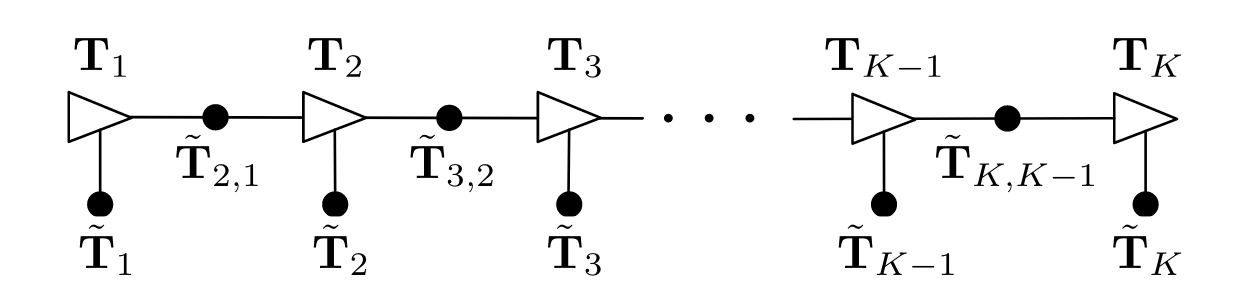
\includegraphics[width=0.6\textwidth]{figures/factor_graph_representation.png}
    \caption{Factor graph representation of the discrete-time estimation problem}
    \label{fig:factor_graph_representation}
\end{figure}
\end{frame}

\section{Trajectory Estimation}
\begin{frame}{Trajectory Estimation Examples}

\begin{figure}
    \centering
    \begin{minipage}{0.48\textwidth}
        \textcolor{myNewColorA}{Discrete-time Trajectory Estimation:}
    \end{minipage}\hfill
    \begin{minipage}{0.48\textwidth}
        \textcolor{myNewColorA}{Continuous-time Trajectory Estimation:}
    \end{minipage}

    \vspace{0.5cm}  % Adjust vertical spacing as needed

    \begin{minipage}{0.48\textwidth}
        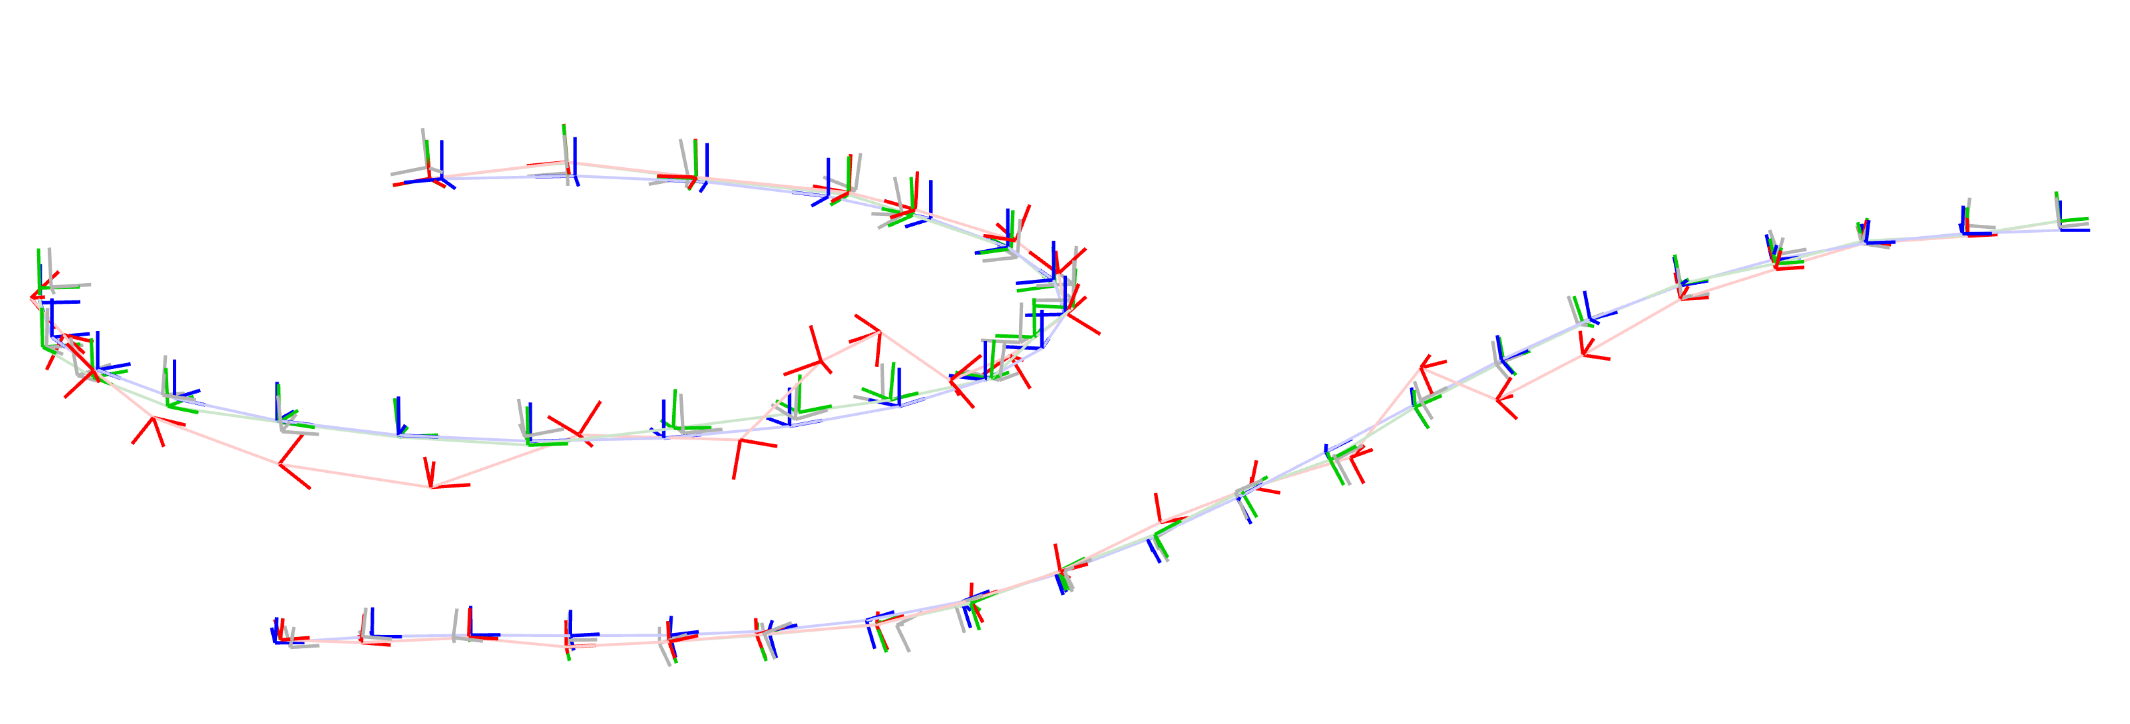
\includegraphics[width=\linewidth]{figures/Discrete-time_Trajectory_Estimation.png}
        \caption{\textit{Discrete-time Trajectory Estimation:} Two examples of discrete-time trajectory estimation where the randomly initialized local solver (red) becomes trapped in a poor local minimum while \textbf{the global solver (green) finds the correct solution}, which is closer to the groundtruth pose (blue).}
    \end{minipage}\hfill
    \begin{minipage}{0.48\textwidth}
        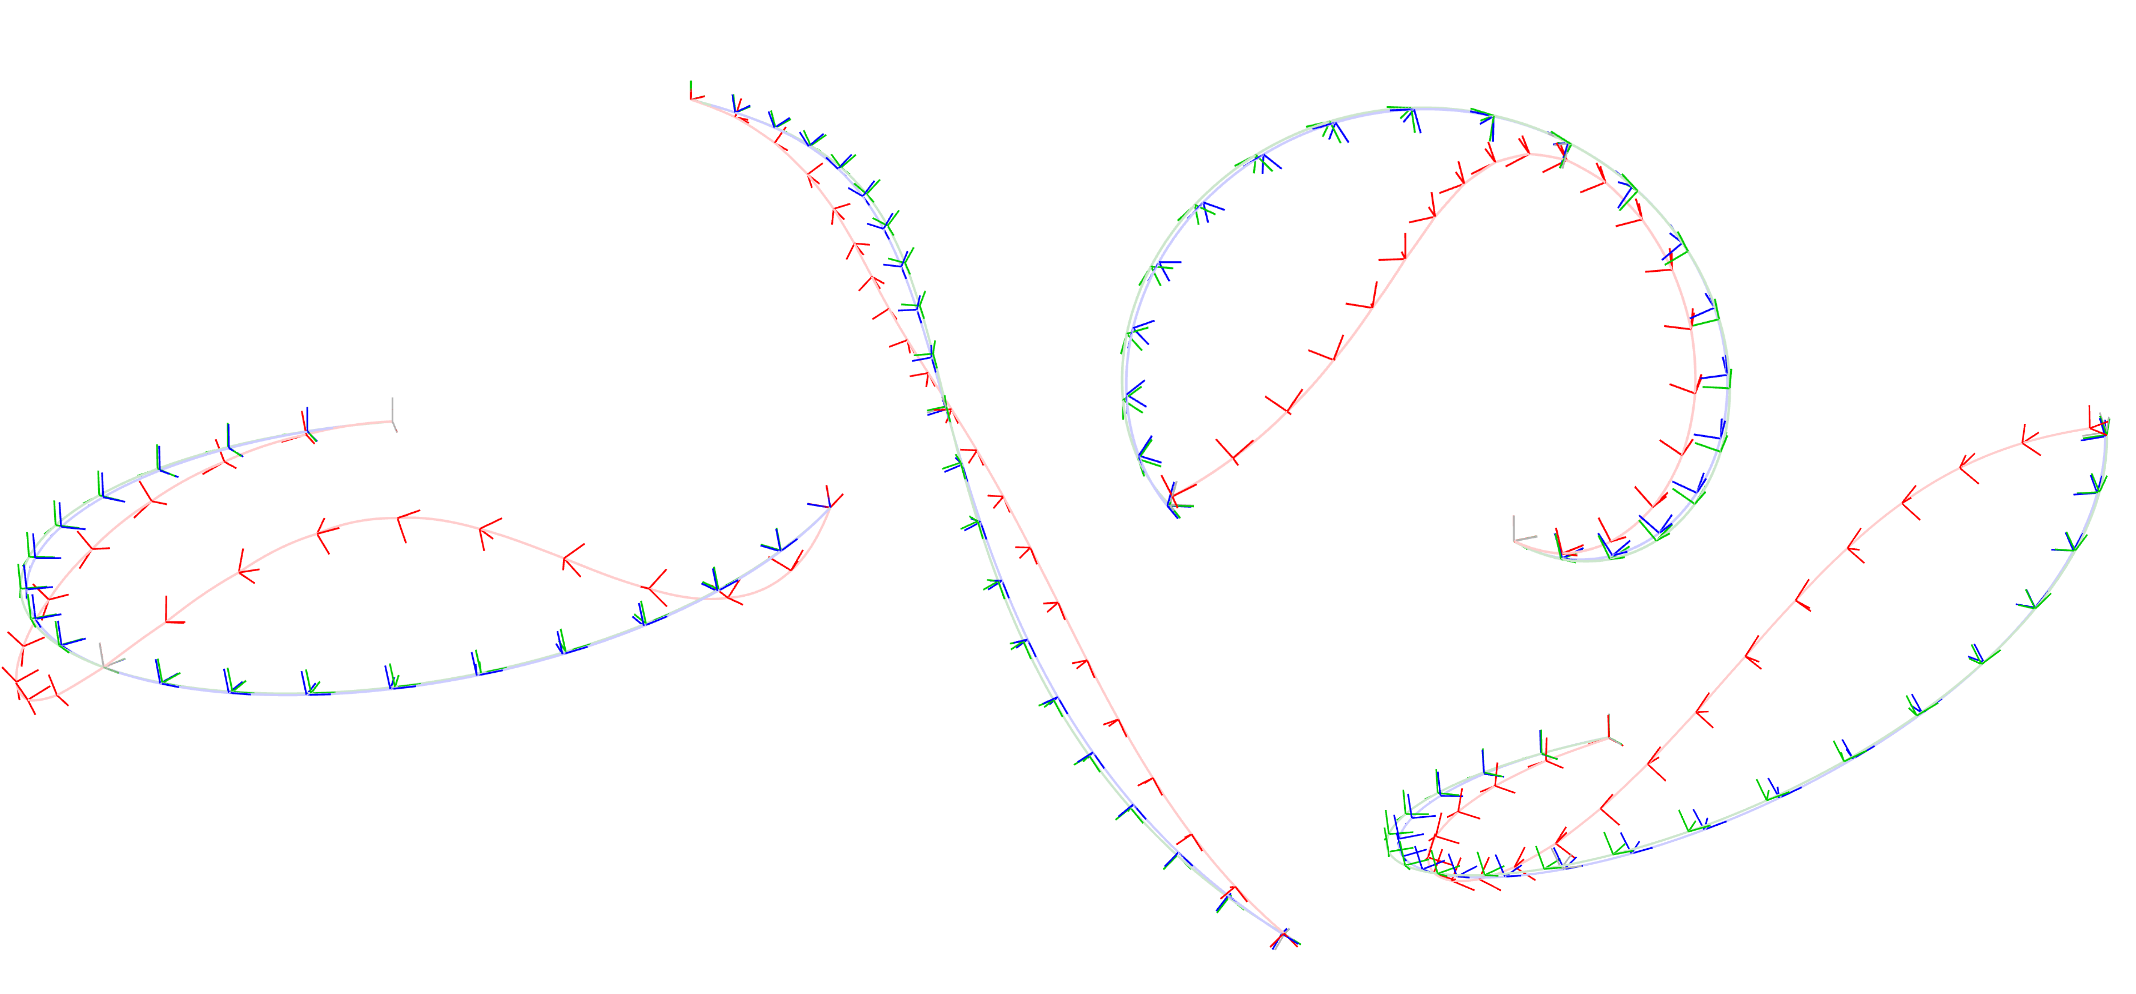
\includegraphics[width=\linewidth]{figures/Continuous-time_Trajectory_Estimation.png}
        \caption{\textit{Continuous-time Trajectory Estimation}: Four examples of continuous-time trajectory estimation where the randomly initialized local solver (red) becomes trapped in a poor local minimum while \textbf{the global solver (green) finds the correct solution}, which is closer to the groundtruth pose (blue). The noisy pose measurements (occurring only at the start, middle, and end of each trajectory) are also shown (grey).}
    \end{minipage}
\end{figure}
\end{frame}

\section{Conclusion and Future Work}
\begin{frame}{Conclusion and Future Work}
This paper presented several new convex relaxations for pose and rotation estimation problems based on the Cayley map. The results indicate that:
\begin{itemize}
    \item[1.] For small sizes, global optimality with realistic amount of noise can be successfully achieved. (which is quite promising as a first step)
    \item[2.] They are still relying on off-the-shelf solvers once the problem has been converted to an SDP, which means that it can not be able to scale up to extremely large state sizes.
\end{itemize}
\vspace{1em}
There are a few possibilities to explore:
\begin{itemize}
    \item[1.] redundant constrains are required to tighten the SDPs, which makes it more challenging to calculate an optimality certificate.
    \item[2.] explore these and other ways of scaling global optimality for \textbf{a larger range of state estimation problems}. 
\end{itemize}
\end{frame}

\section*{Acknowledgement}  
\begin{frame}
\centering
\textcolor{myNewColorA}{\fontsize{40pt}{50pt}\selectfont Thank You!}
\end{frame}

\end{document}
